\documentclass[aspectratio=169]{beamer}
\usetheme{metropolis}

\usepackage[english]{babel}

\usepackage{booktabs}
\usepackage[scale=2]{ccicons}
\usepackage[framemethod=tikz]{mdframed}

\usepackage{graphicx}
\usepackage{pgfpages}
\usepackage{appendixnumberbeamer}
\usepackage{pgfplots}

\usepackage{xcolor}
\usepackage{xspace}
\newcommand{\themename}{\textbf{\textsc{metropolis}}\xspace}

\definecolor{titleframecolor}{HTML}{23373B}
\definecolor{titlebackgroundcolor}{HTML}{FAFAFA}

%Information to be included in the title page:
\title{Why Are You So Busy?}
\subtitle{An Analog System for the Digital Age}
\author{Ritger Teunissen (ritger@hack42.nl)}
\institute{Hack42, Arnhem}
\date{\today}
%\setbeamertemplate{frame footer}{\today}
%\setbeameroption{show notes}
%\setbeameroption{show notes on second screen}

\newmdenv[tikzsetting={draw=titleframecolor,fill=titlebackgroundcolor,fill opacity=0.8, line width=1pt},
      backgroundcolor=none,leftmargin=0,rightmargin=0,innertopmargin=7pt]
      {titlebox}

\begin{document}
    \maketitle

    %\begin{frame}{Table of Contents}
    %    \setbeamertemplate{section in toc}[sections numbered]
    %    \tableofcontents[hideallsubsections]
    %\end{frame}

    \section{So, Why Are You So Busy?}

    {
    \usebackgroundtemplate{
\includegraphics[height=\paperheight]{images/01_good_news.jpg}}
    \begin{frame}{Good News Everyone!}
        \begin{titlebox}
            \centering
            {\alert{Statistically} speaking, you're about as busy as anyone used
            to be \\ (if you're Dutch)}
        \end{titlebox}
    \end{frame}
    }

    \section{`Het Tijdsbestedingsonderzoek'}

    {
    \usebackgroundtemplate{
\includegraphics[height=\paperheight]{images/02_good_news_opaque.jpg}}
    \begin{frame}{Overview}
        \begin{itemize}
            \item Dutch people have been keeping a diary (for a singe week) since 1975
            \item On average \textasciitilde2500 people write a usable diary
            \item Results are compiled and corrected for use
        \end{itemize}
    \end{frame}
    }

    {
    \usebackgroundtemplate{
\includegraphics[height=\paperheight]{images/02_good_news_opaque.jpg}}
    \begin{frame}{Compare (1)}
        \begin{figure}
            \begin{tikzpicture}
                \begin{axis}[
                    mbarplot,
                    /pgf/number format/1000 sep={},
                    xlabel={Years},
                    ylabel={Hours},
                    ymin=40,
                    ymax=48,
                    width=0.9\textwidth,
                    height=7cm,
                    symbolic x coords={1975,1980,1985,1990,1995,2000,2005,2006,2011},
                    xtick=data,
                    bar width=0.4cm
                    ]

                    \addplot plot coordinates {(1975, 40.7) (1980, 40.8) (1985, 40.7) (1990, 42.0) (1995, 42.6) (2000, 43.9) (2005, 44.3) (2006, 42.8) (2011, 41.2)};
                    \legend{Gotta Do, All You}
                \end{axis}
            \end{tikzpicture}
        \end{figure}
    \end{frame}
    }

    {
    \usebackgroundtemplate{
\includegraphics[height=\paperheight]{images/02_good_news_opaque.jpg}}
    \begin{frame}{Compare (2)}
        \begin{figure}
            \begin{tikzpicture}
                \begin{axis}[
                    mbarplot,
                    /pgf/number format/1000 sep={},
                    xlabel={Years},
                    ylabel={Hours},
                    ymin=40,
                    ymax=48,
                    width=0.9\textwidth,
                    height=7cm,
                    symbolic x coords={1975,1980,1985,1990,1995,2000,2005,2006,2011},
                    xtick=data,
                    bar width=0.4cm
                    ]

                    \addplot plot coordinates {(1975, 40.7) (1980, 40.8) (1985, 40.7) (1990, 42.0) (1995, 42.6) (2000, 43.9) (2005, 44.3) (2006, 42.8) (2011, 41.2)};
                    \addplot plot coordinates {(1975, 47.9) (1980, 47.0) (1985, 49.0) (1990, 47.2) (1995, 47.3) (2000, 44.8) (2005, 44.7) (2006, 46.9) (2011, 47.8)};
                    \legend{Gotta Do, All You}
                \end{axis}
            \end{tikzpicture}
        \end{figure}
    \end{frame}
    }

    \begin{frame}[standout]
        Questions?
    \end{frame}

    \section{Why Do You \emph{Feel} So Busy?}

    {
    \usebackgroundtemplate{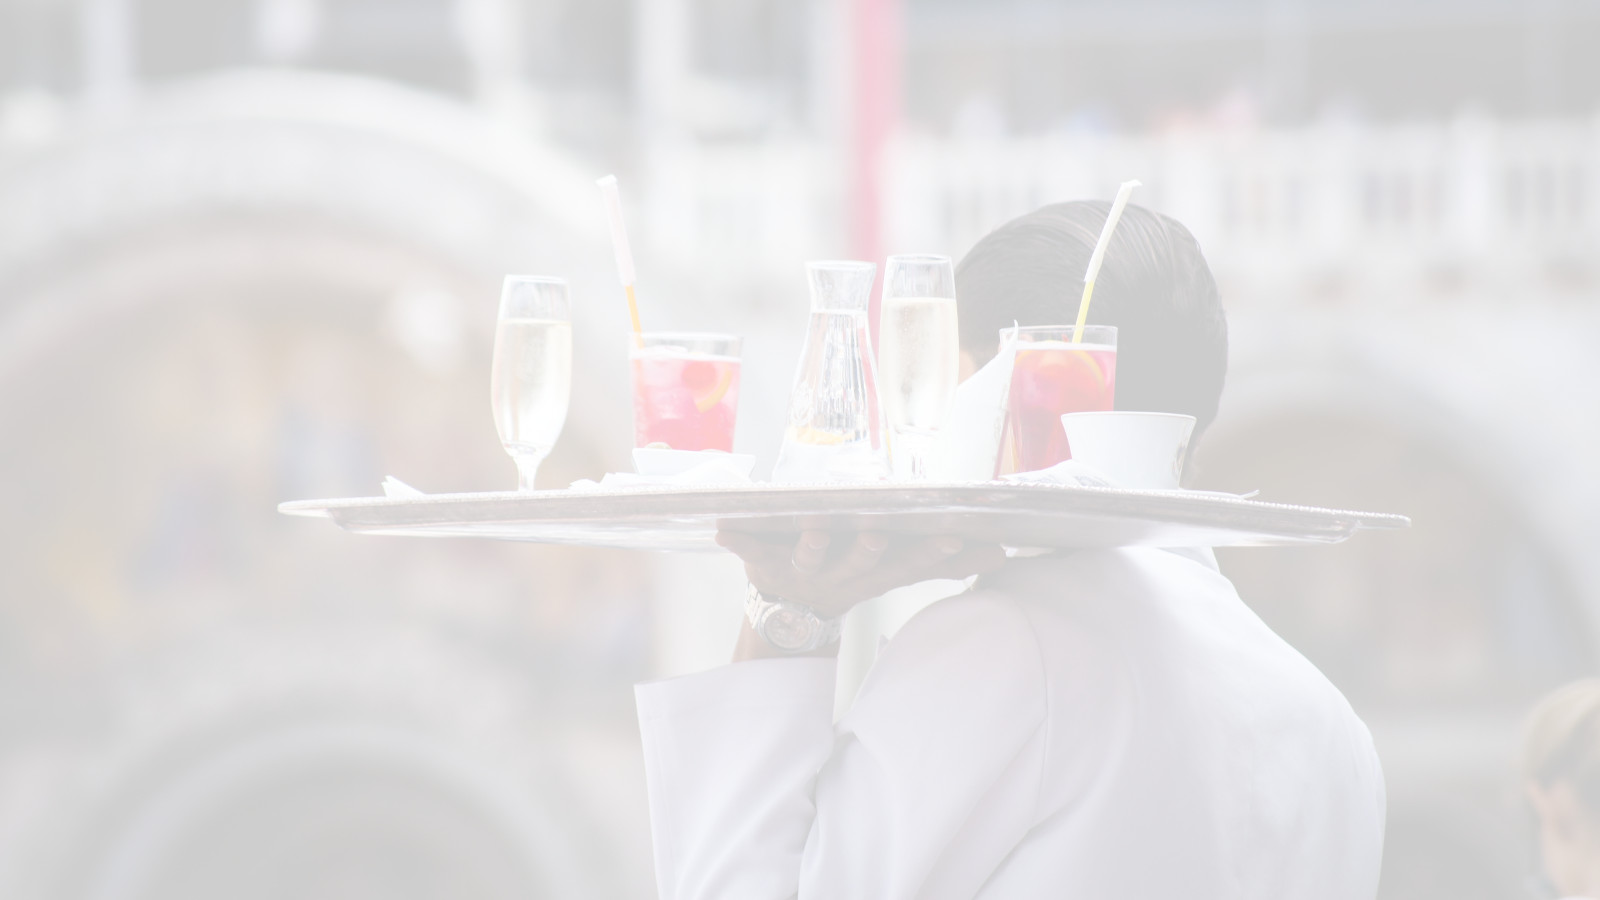
\includegraphics[height=\paperheight]{images/07_waiter_opaque.jpg}}
    \begin{frame}{The Zeigarnik Effect}
        \begin{columns}[T,onlytextwidth]
            \column{0.5\textwidth}
                \vspace{3em}
                \begin{itemize}
                    \item Named after \emph{Bluma Zeigarnik} (research published in 1927)
                    \item First noticed in a waiter taking her order
                    \item Theory: Unfinished tasks linger, finished tasks get forgotten
                    \item Assumes a limited amount of \alert{`cognitive bandwidth'}
                \end{itemize}
            \column{0.5\textwidth}
                \begin{figure}[h]
                    \centering
                    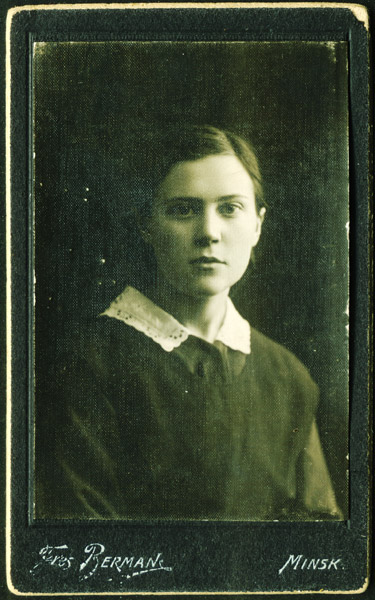
\includegraphics[width=90pt,keepaspectratio]{images/08_bluma_zeigarnik.jpg}
                    \caption{Wikimedia Commons}
                \end{figure}
        \end{columns}
    \end{frame}
    }

    {
    \usebackgroundtemplate{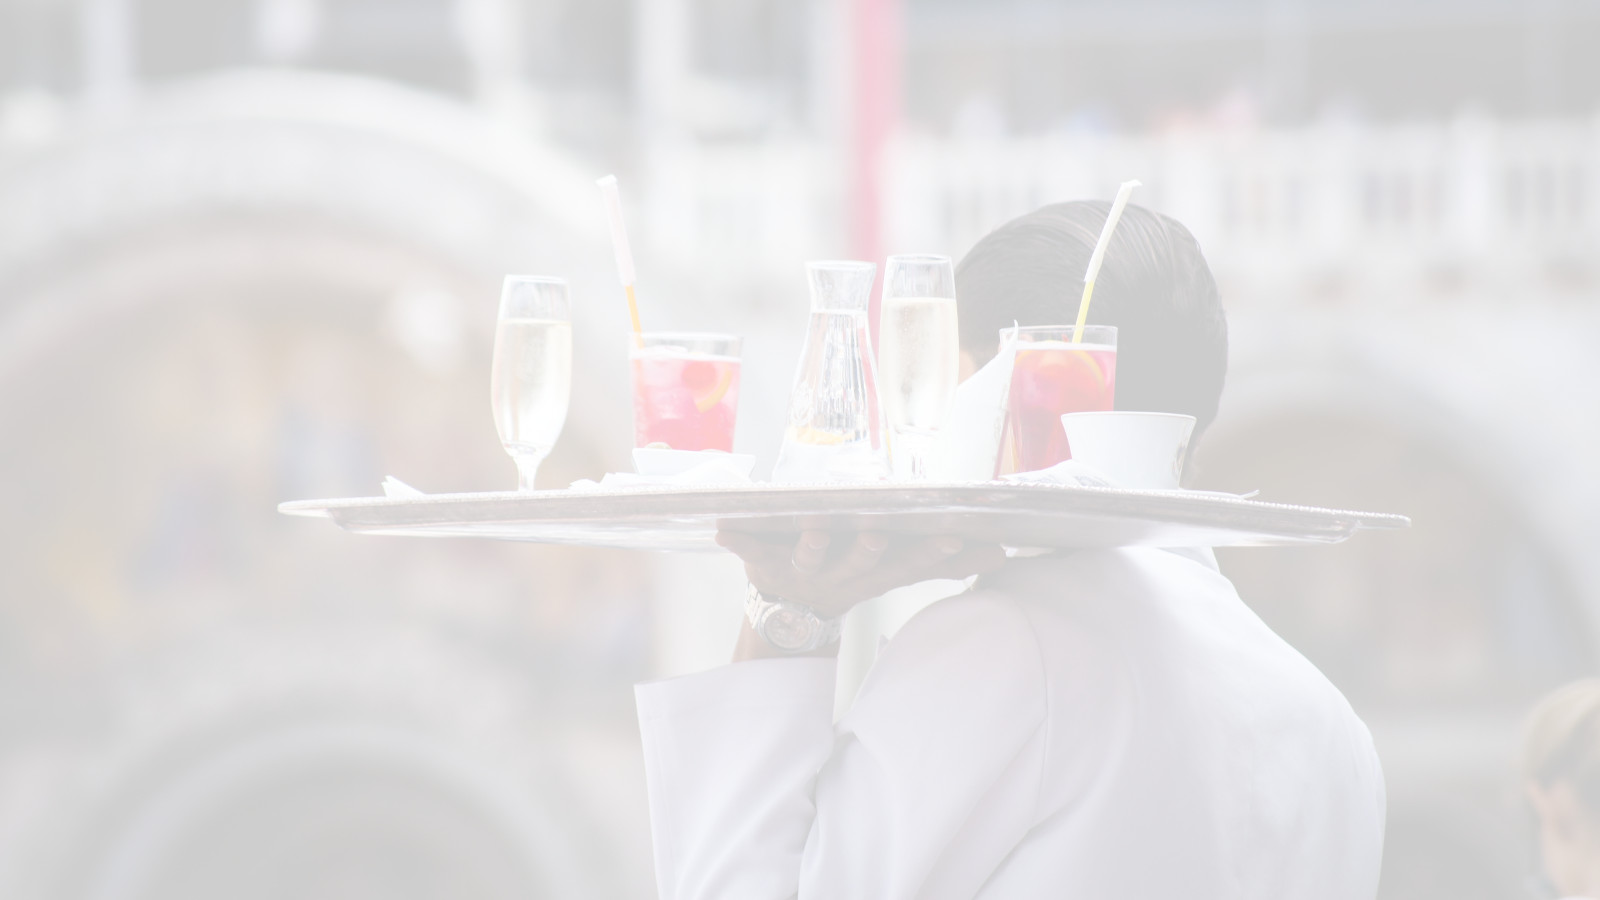
\includegraphics[height=\paperheight]{images/07_waiter_opaque.jpg}}
    \begin{frame}{Maybe not \ldots}
        \begin{itemize}
            \item Original research on a limited number of subjects
            \item Could not be reproduced in more extensive research\footnote{van Bergen, 1968}
            \pause
            \item So what else?
        \end{itemize}
        \note[item]{So if not the Zeigarnik Effect, what is the cause?}
    \end{frame}
    }

    \begin{frame}[standout]
        Spoiler: There is no `one size fits all'
    \end{frame}

    {
    \usebackgroundtemplate{
\includegraphics[height=\paperheight]{images/03_mythbusters.jpg}}
    \begin{frame}{Remember Kids \ldots}
        \begin{titlebox}
            \centering
            `The only difference between screwing around and science is \alert{writing it down}.'
        \end{titlebox}
    \end{frame}
    }

    \section{An Analog System for the Digital Age}

    {
    \usebackgroundtemplate{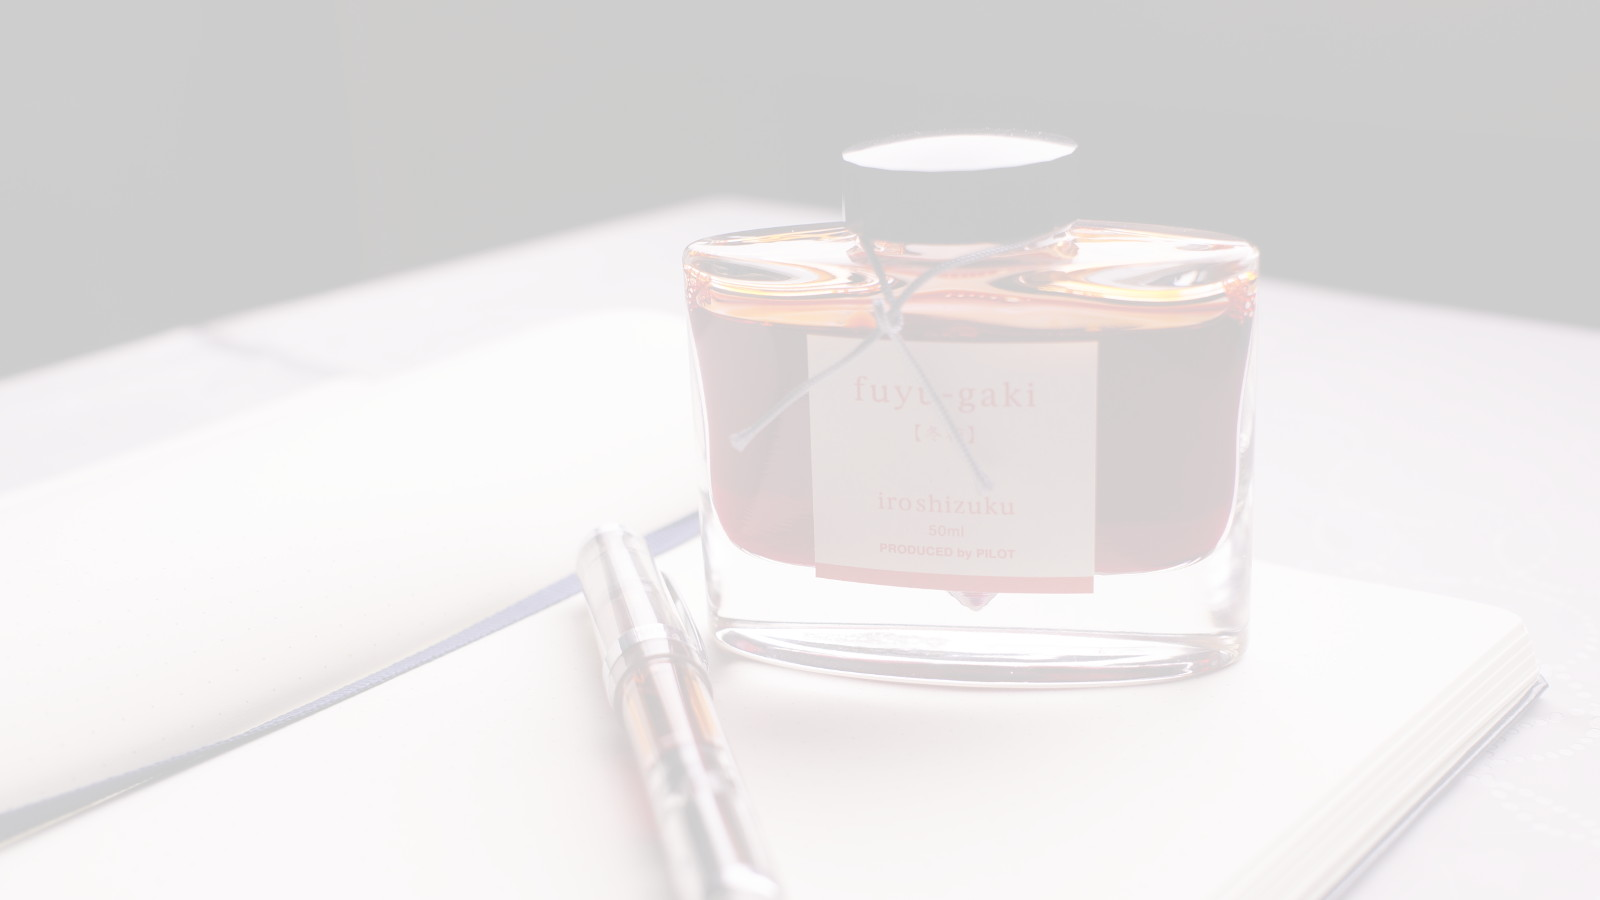
\includegraphics[height=\paperheight]{images/10_notebook_opaque.jpg}}
    \begin{frame}{Bullet Journal}
        \begin{itemize}
            \item Ryder Carroll (bulletjournal.com)
            \item \alert{Track the past}
            \item Order the present
        \end{itemize}
    \end{frame}
    }

    {
    \usebackgroundtemplate{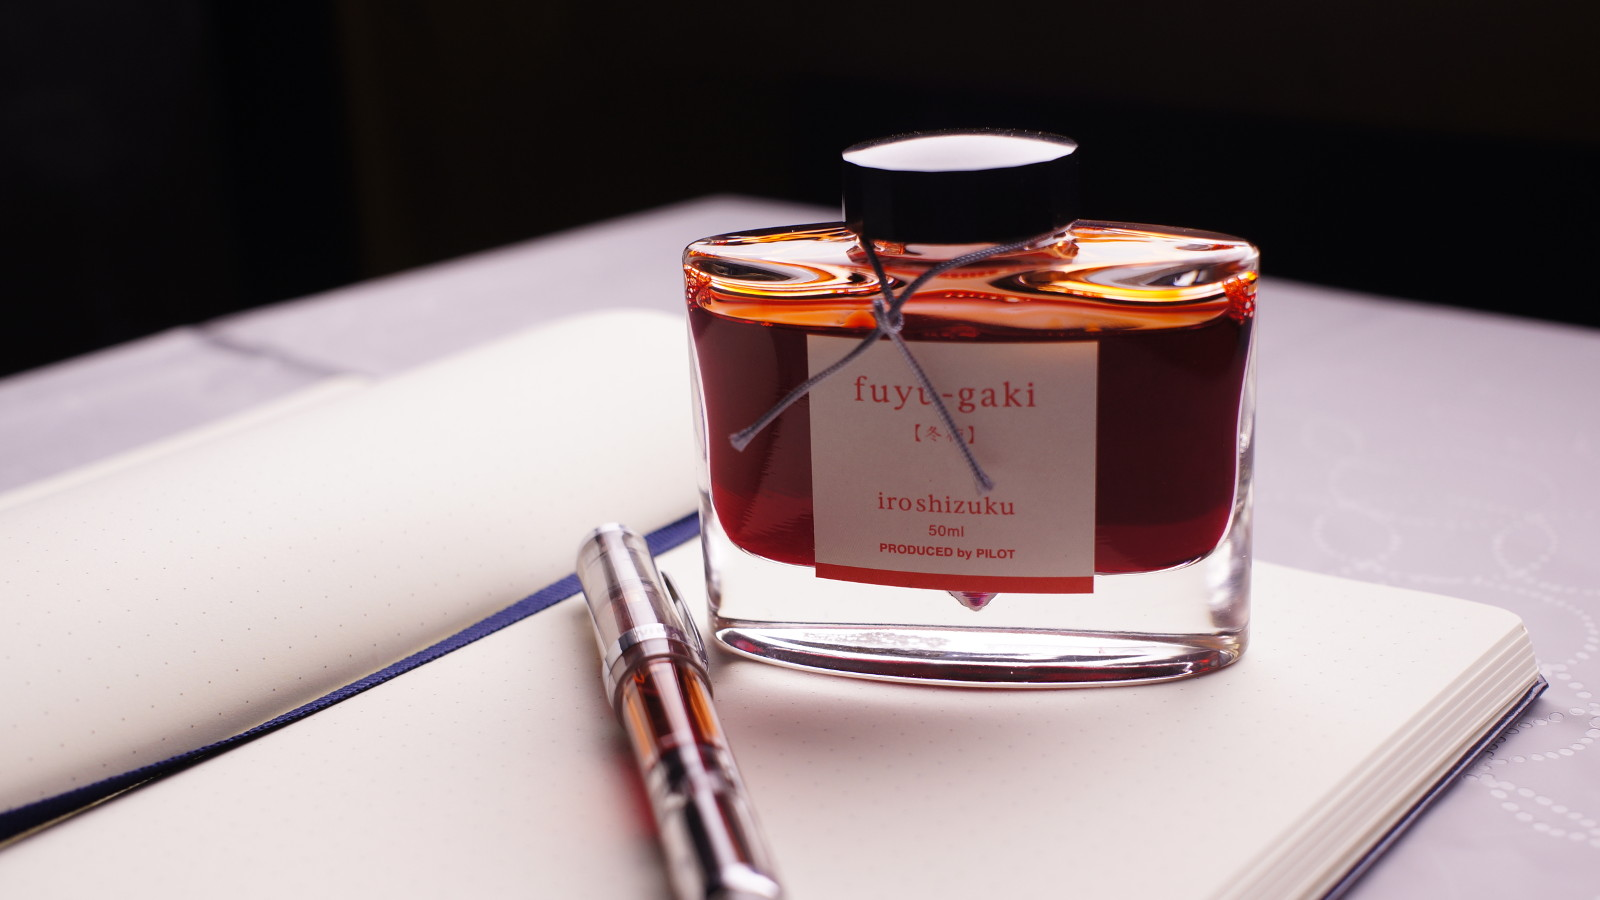
\includegraphics[height=\paperheight]{images/09_notebook.jpg}}
    \begin{frame}{Accessorise}
        \begin{titlebox}
            \centering
            Get a notebook and a pen
        \end{titlebox}
    \end{frame}
    }

    {
    \usebackgroundtemplate{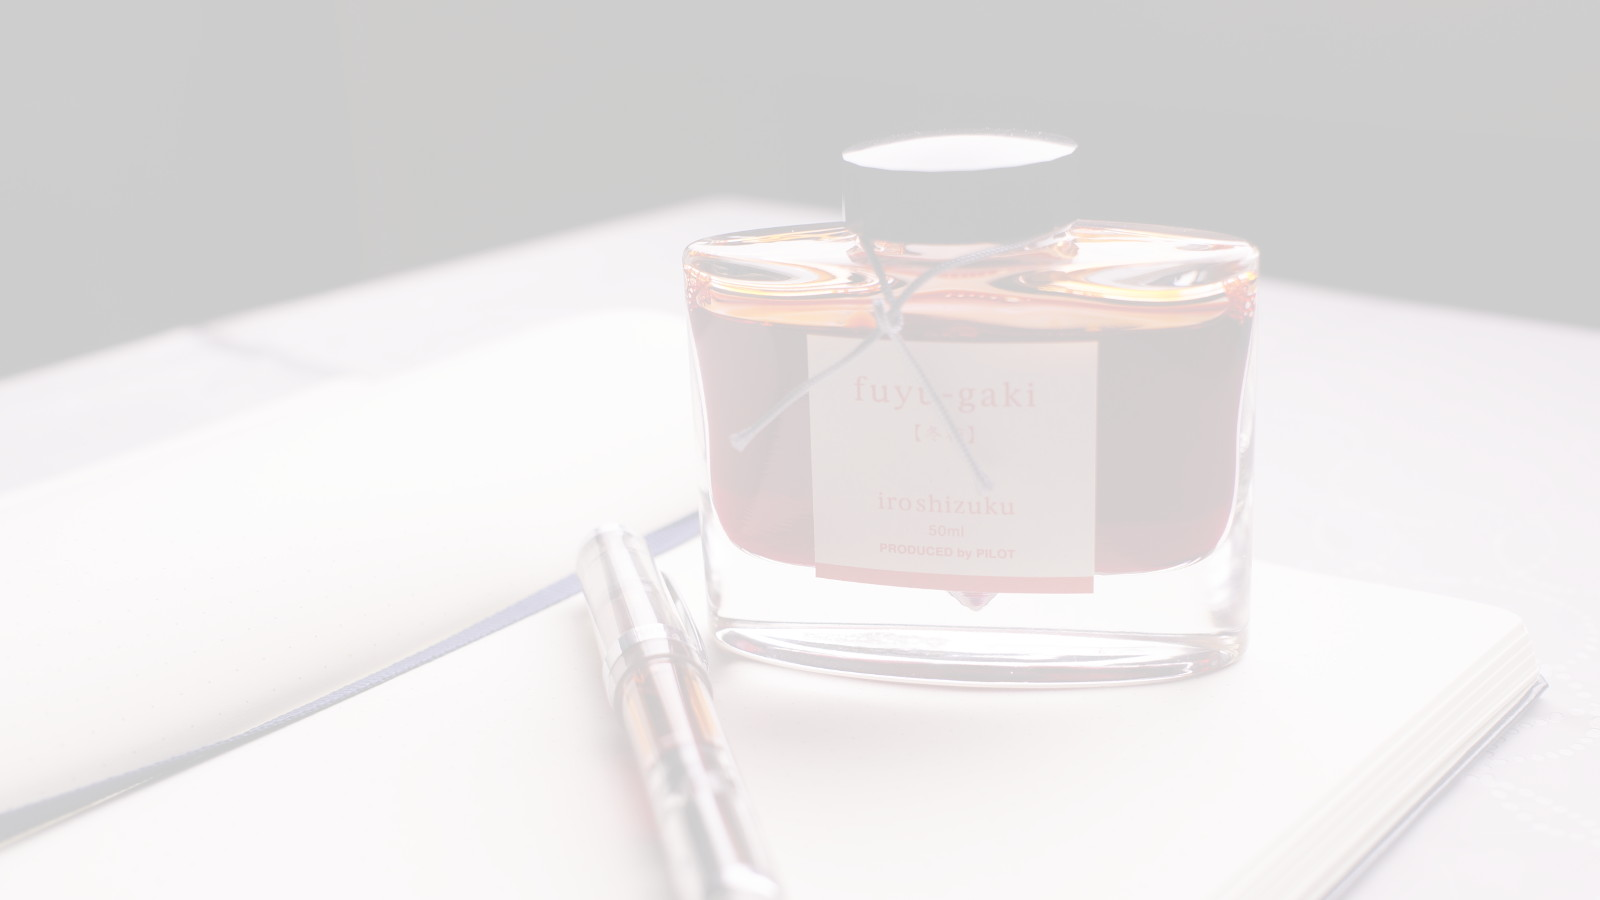
\includegraphics[height=\paperheight]{images/10_notebook_opaque.jpg}}
    \begin{frame}{Why Do This on Paper?}
        \begin{itemize}
            \item Intentionally slows you down, forces you to think
            \item Writing helps with processing information\footnote{Princeton et.al.}
            \pause
            \item No distractions!
        \end{itemize}
    \end{frame}
    }

    {
    \usebackgroundtemplate{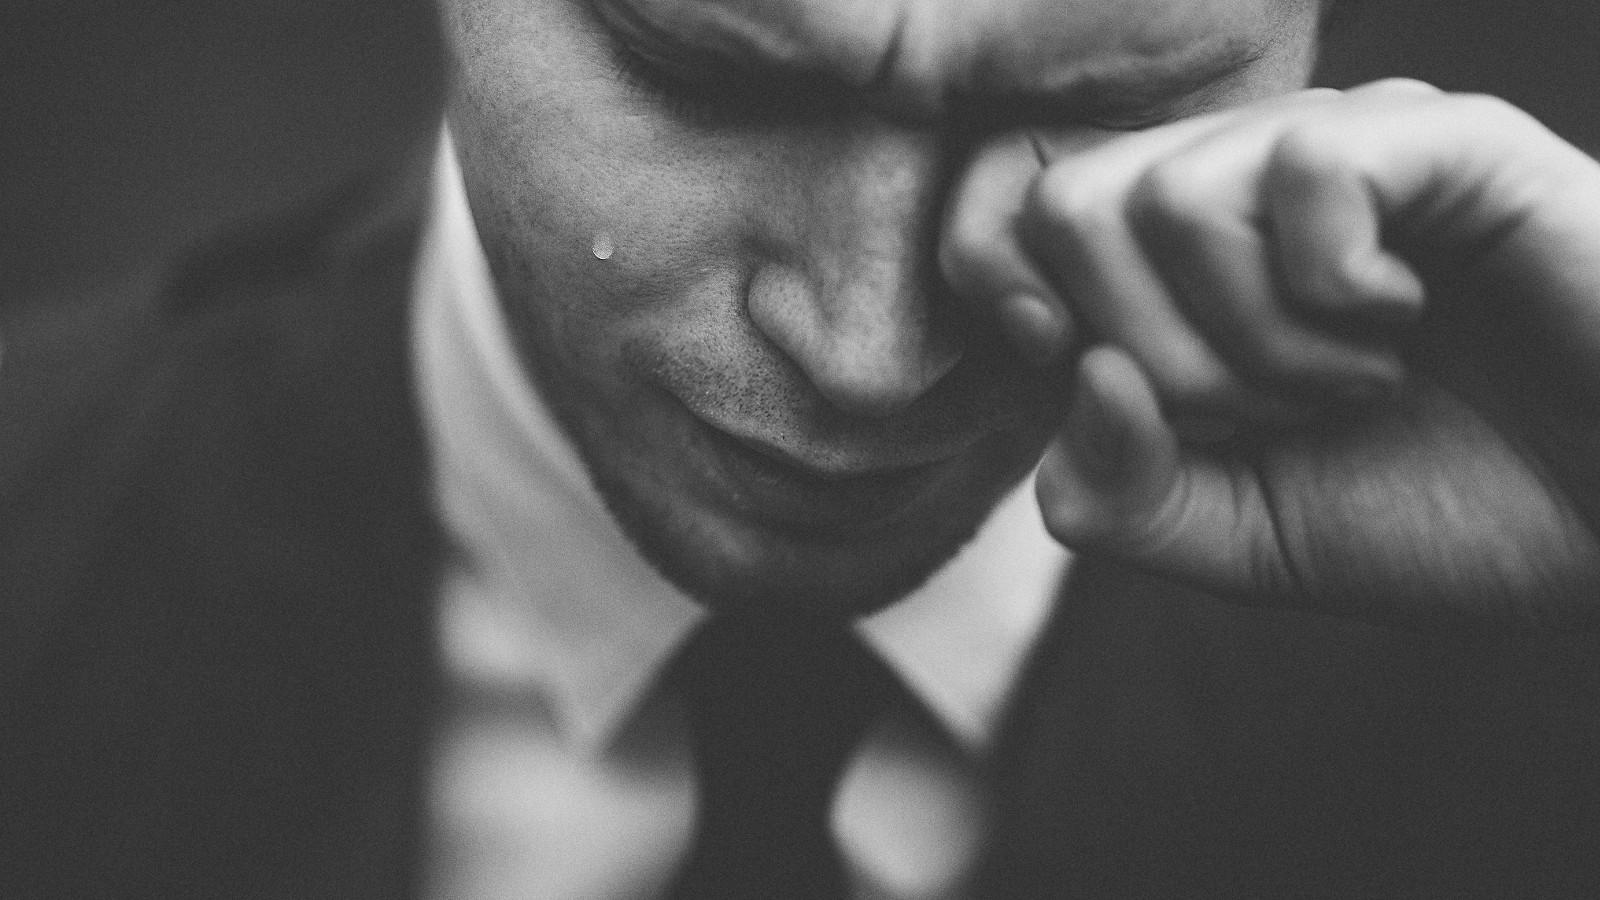
\includegraphics[height=\paperheight]{images/11_crying.jpg}}
    \begin{frame}%{S\'o\'o\'o\'o Busy \ldots}
        \begin{titlebox}
            \centering
            But I'm too busy to write things down!
        \end{titlebox}
    \end{frame}
    }

    \section{Starting Your Bullet Journal}

    {
    \usebackgroundtemplate{
\includegraphics[height=\paperheight]{images/12_monthly_log.jpg}}
    \begin{frame}{Monthly Log}
    \end{frame}
    }

    {
    \usebackgroundtemplate{
\includegraphics[height=\paperheight]{images/13_monthly_log.jpg}}
    \begin{frame}{Monthly Log}
    \end{frame}
    }

    {
    \usebackgroundtemplate{
\includegraphics[height=\paperheight]{images/14_monthly_log.jpg}}
    \begin{frame}{Monthly Log (Fancy!)}
    \end{frame}
    }

    {
    \usebackgroundtemplate{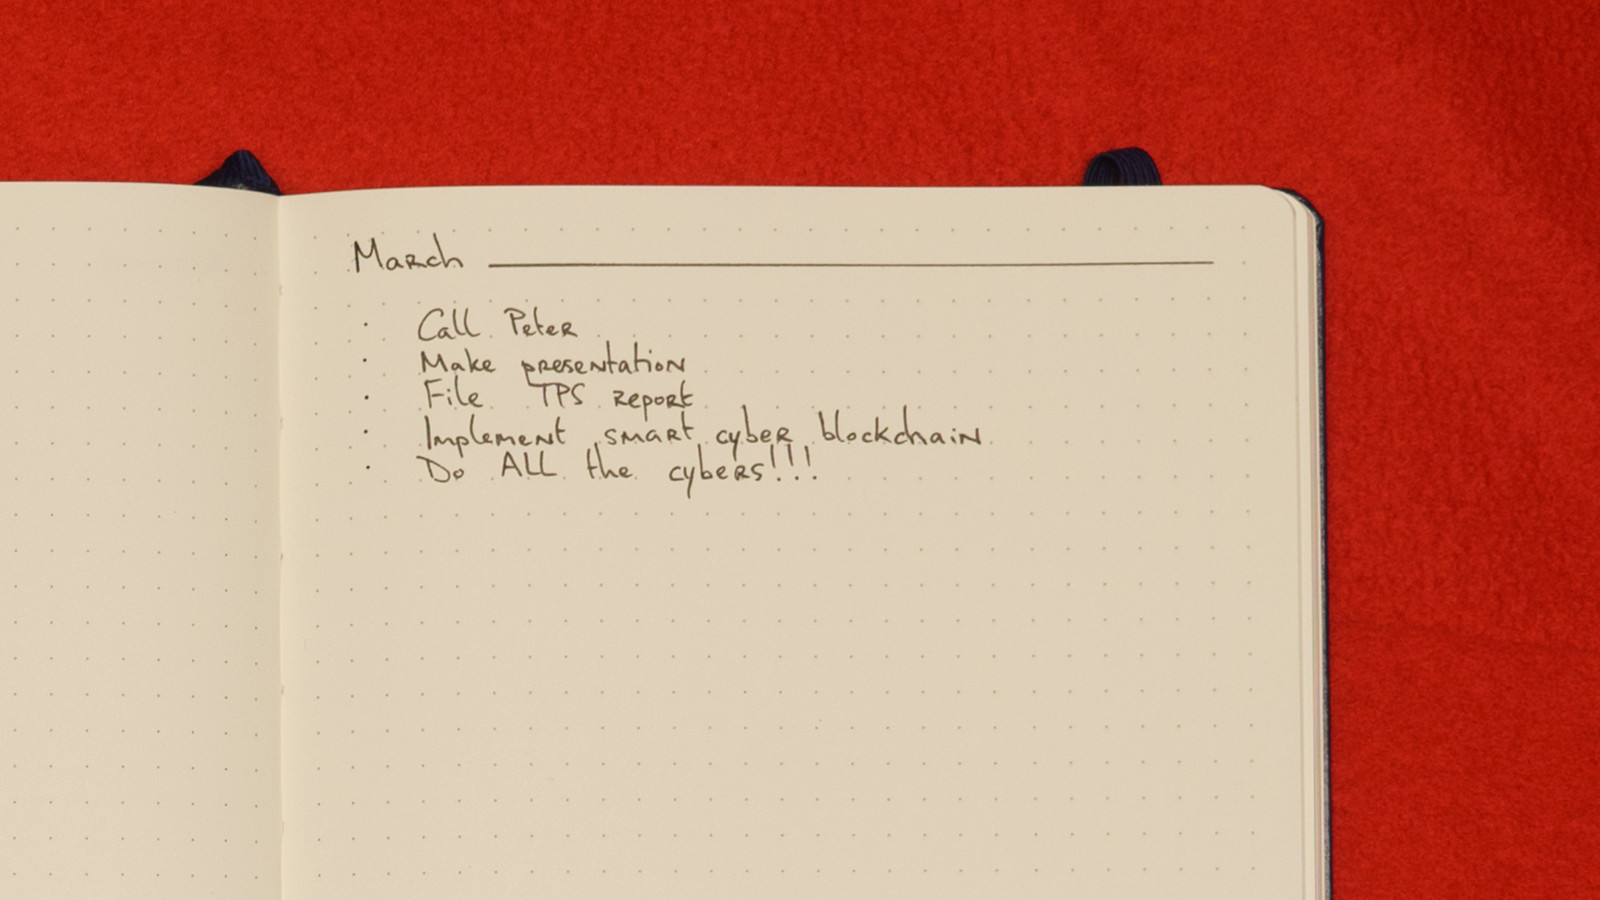
\includegraphics[height=\paperheight]{images/15_monthly_log.jpg}}
    \begin{frame}{Monthly Log}
    \end{frame}
    }

    {
    \usebackgroundtemplate{
\includegraphics[height=\paperheight]{images/12_monthly_log.jpg}}
    \begin{frame}{Daily Log}
    \end{frame}
    }

    {
    \usebackgroundtemplate{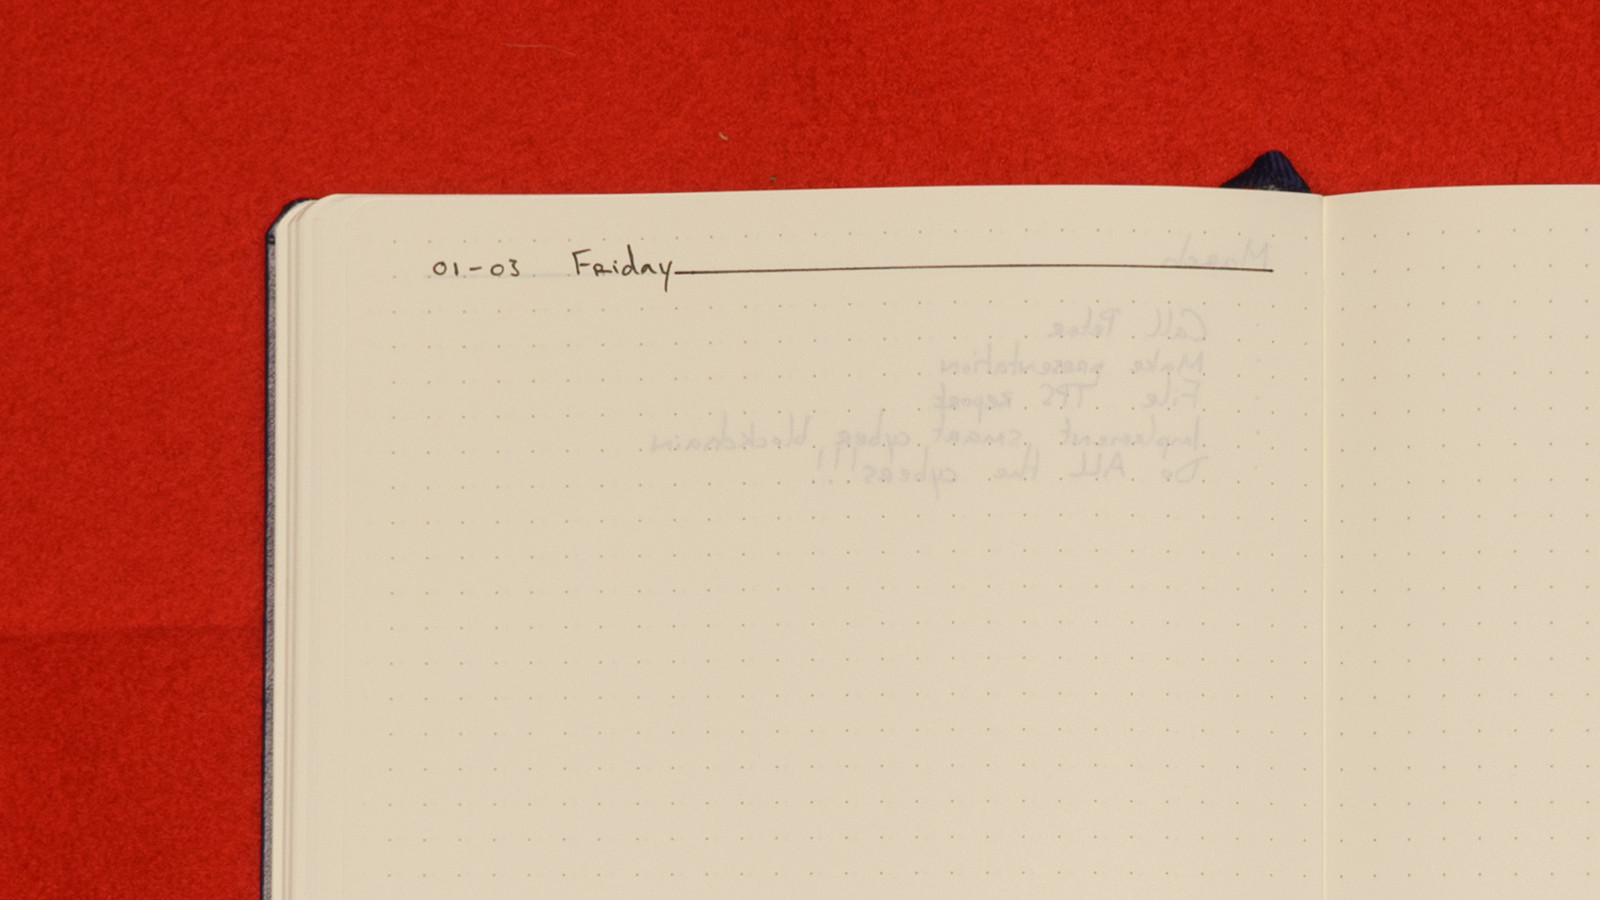
\includegraphics[height=\paperheight]{images/16_daily_log.jpg}}
    \begin{frame}{Daily Log}
    \end{frame}
    }

    {
    \usebackgroundtemplate{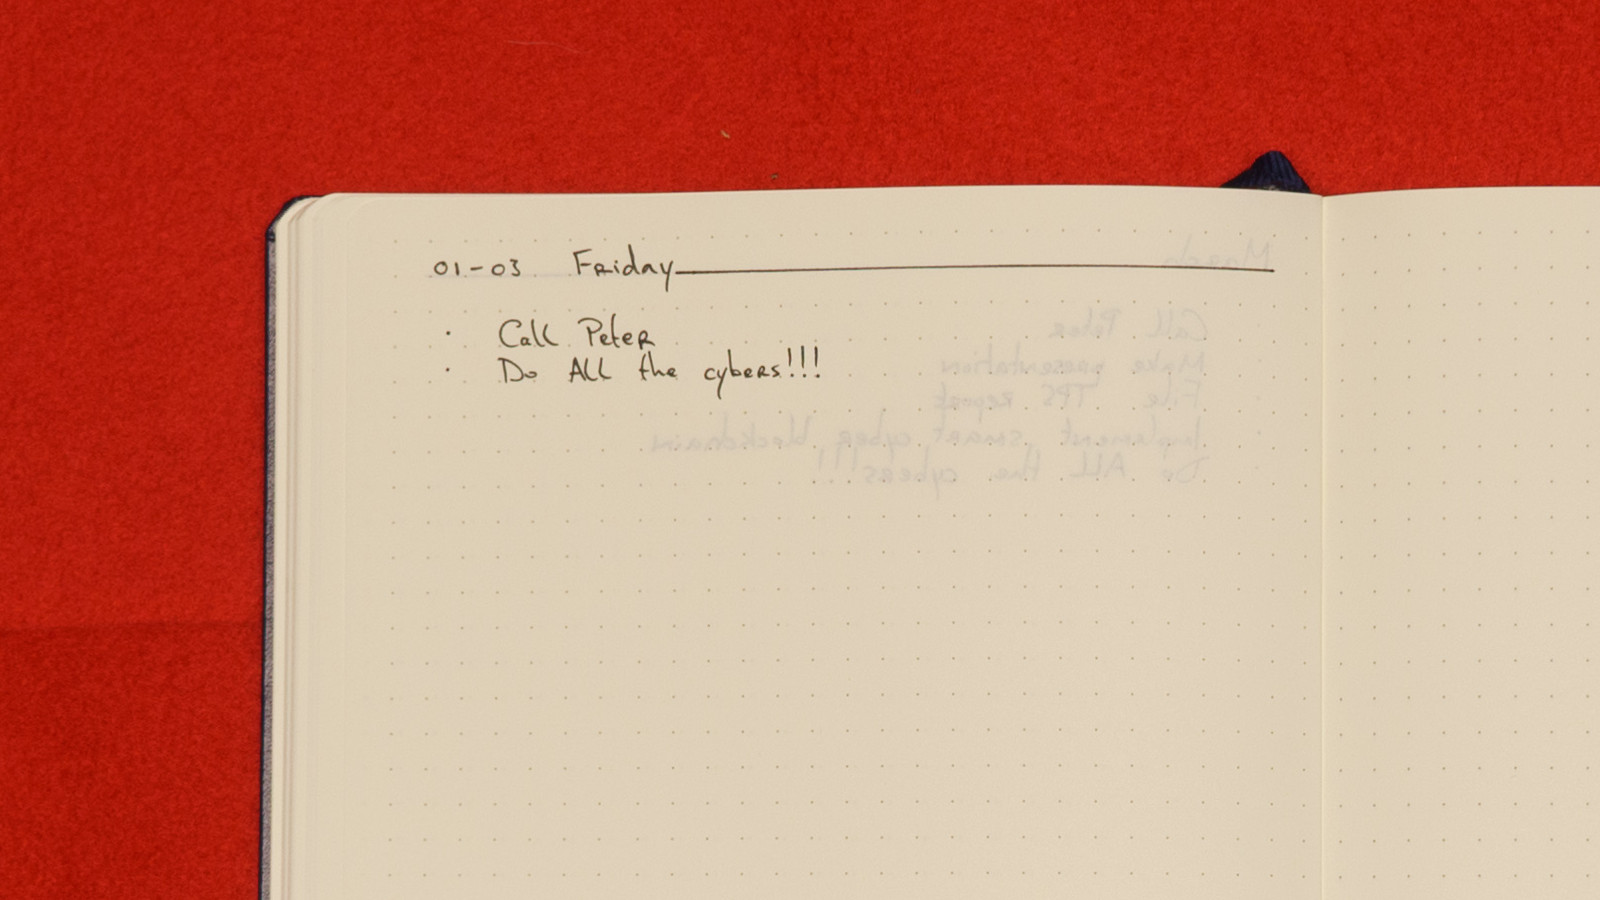
\includegraphics[height=\paperheight]{images/17_daily_log.jpg}}
    \begin{frame}{Daily Log}
    \end{frame}
    }

    {
    \usebackgroundtemplate{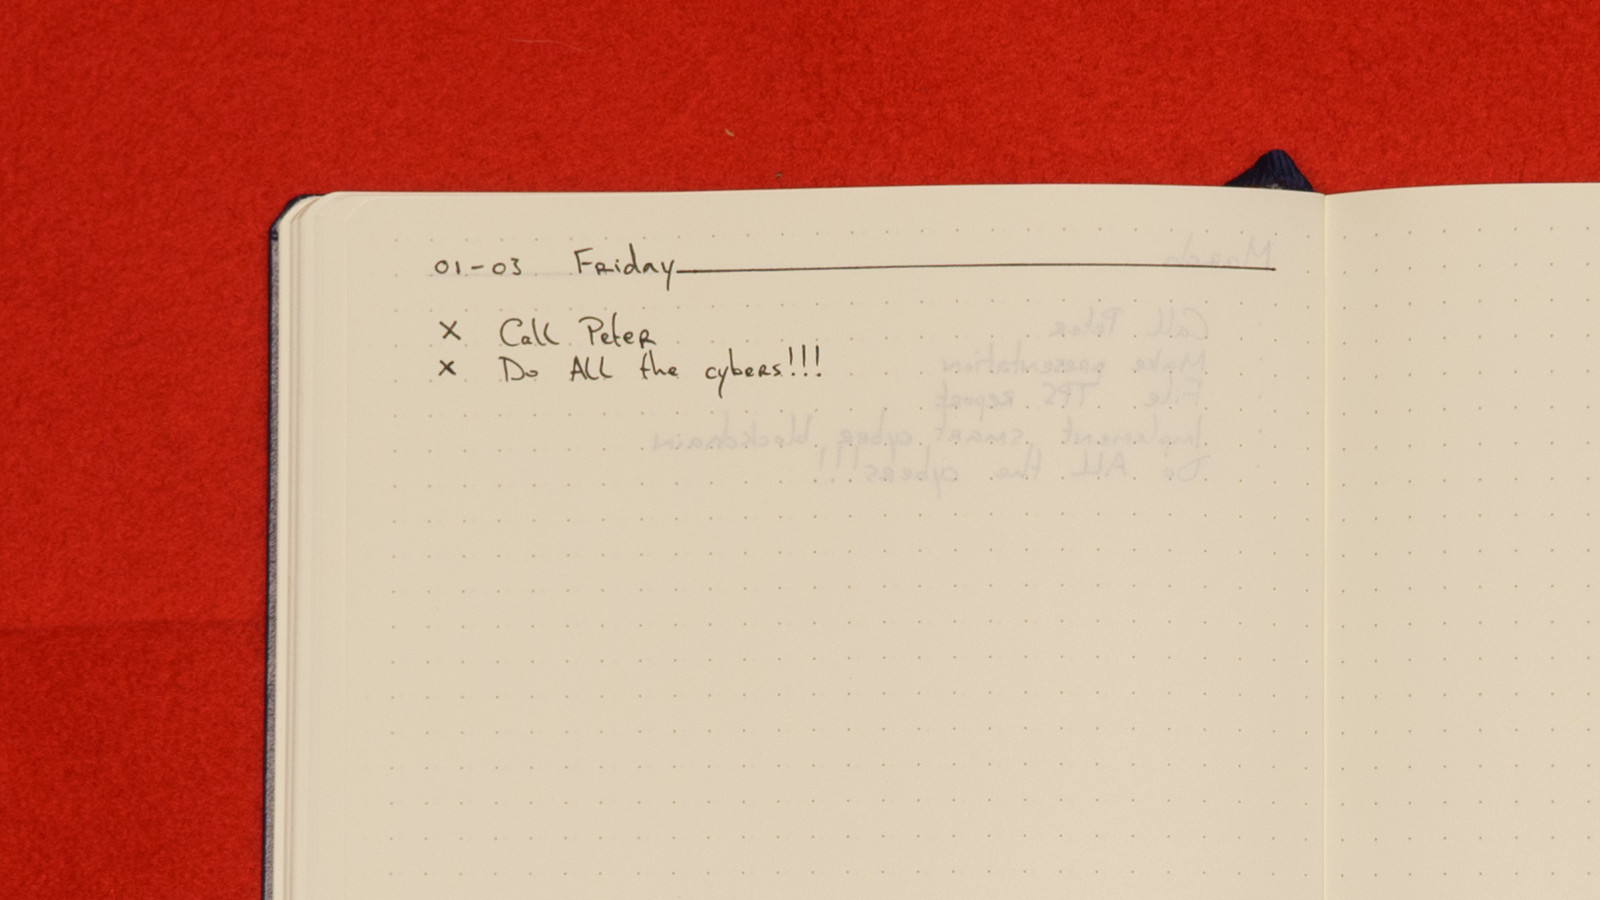
\includegraphics[height=\paperheight]{images/18_daily_log.jpg}}
    \begin{frame}{Daily Log}
    \end{frame}
    }

    {
    \usebackgroundtemplate{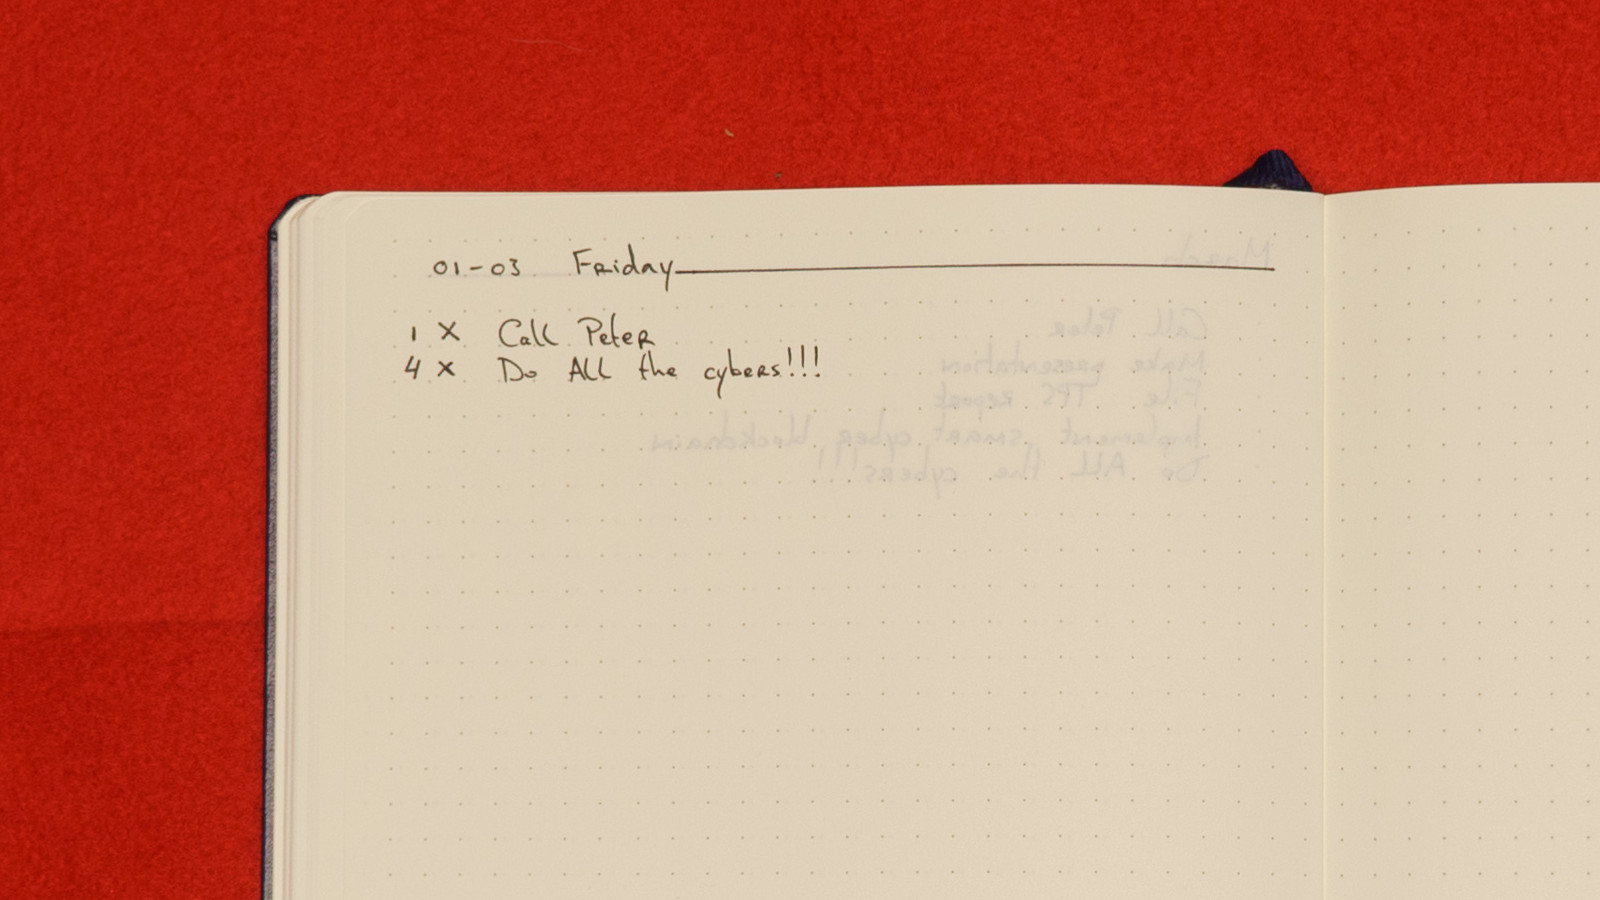
\includegraphics[height=\paperheight]{images/19_daily_log.jpg}}
    \begin{frame}{Daily Log}
    \end{frame}
    }

    {
    \usebackgroundtemplate{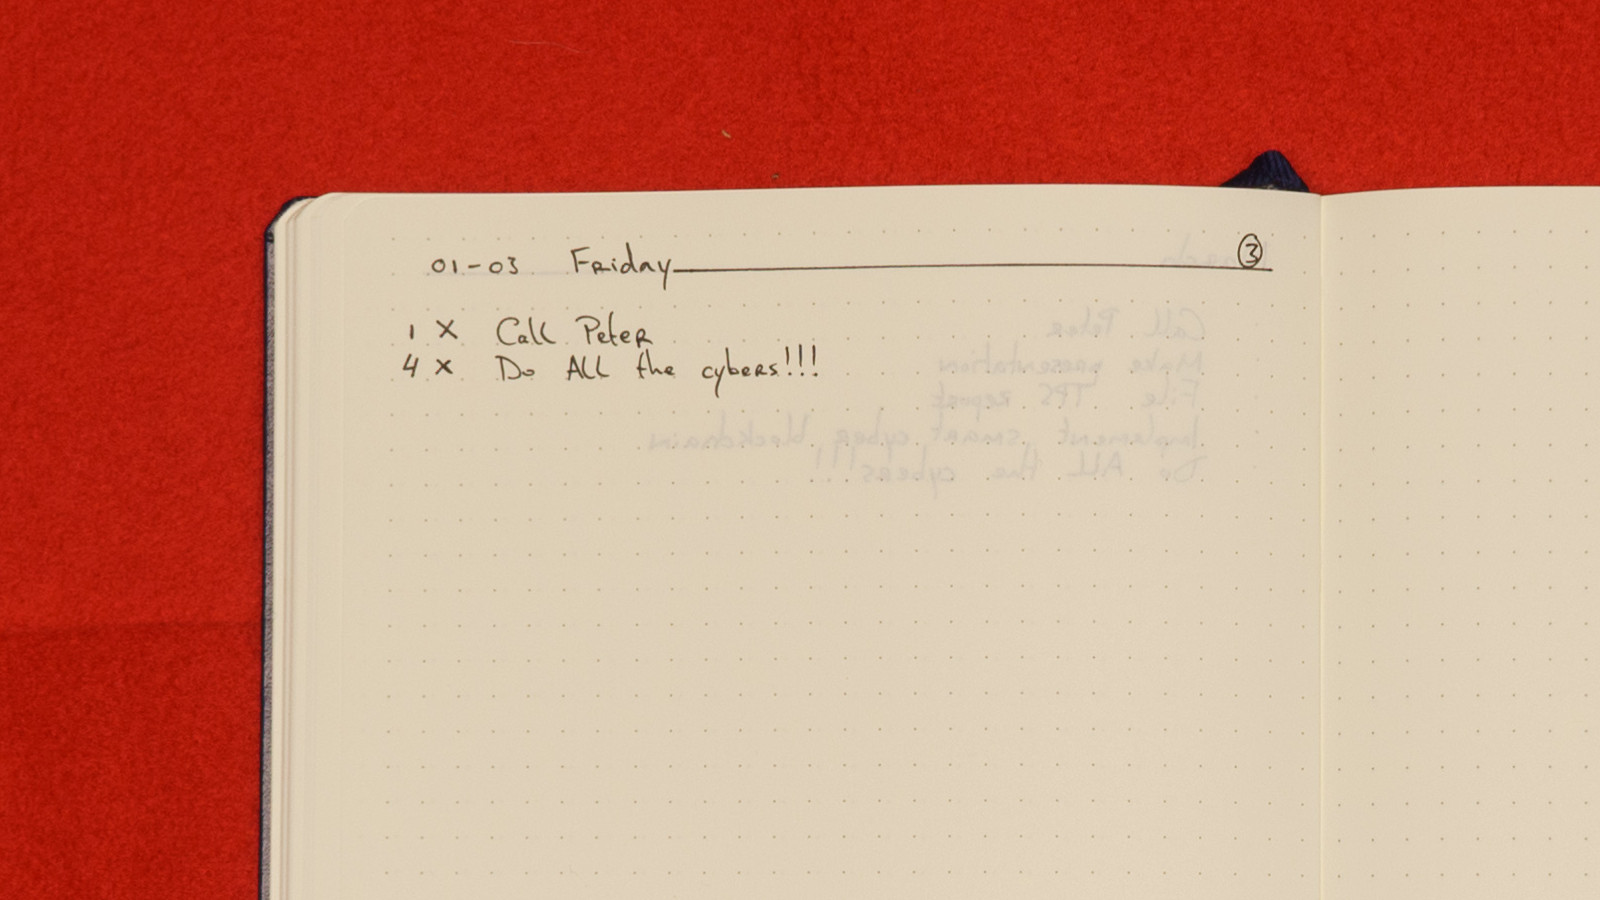
\includegraphics[height=\paperheight]{images/20_daily_log.jpg}}
    \begin{frame}{Daily Log}
    \end{frame}
    }

    {
    \usebackgroundtemplate{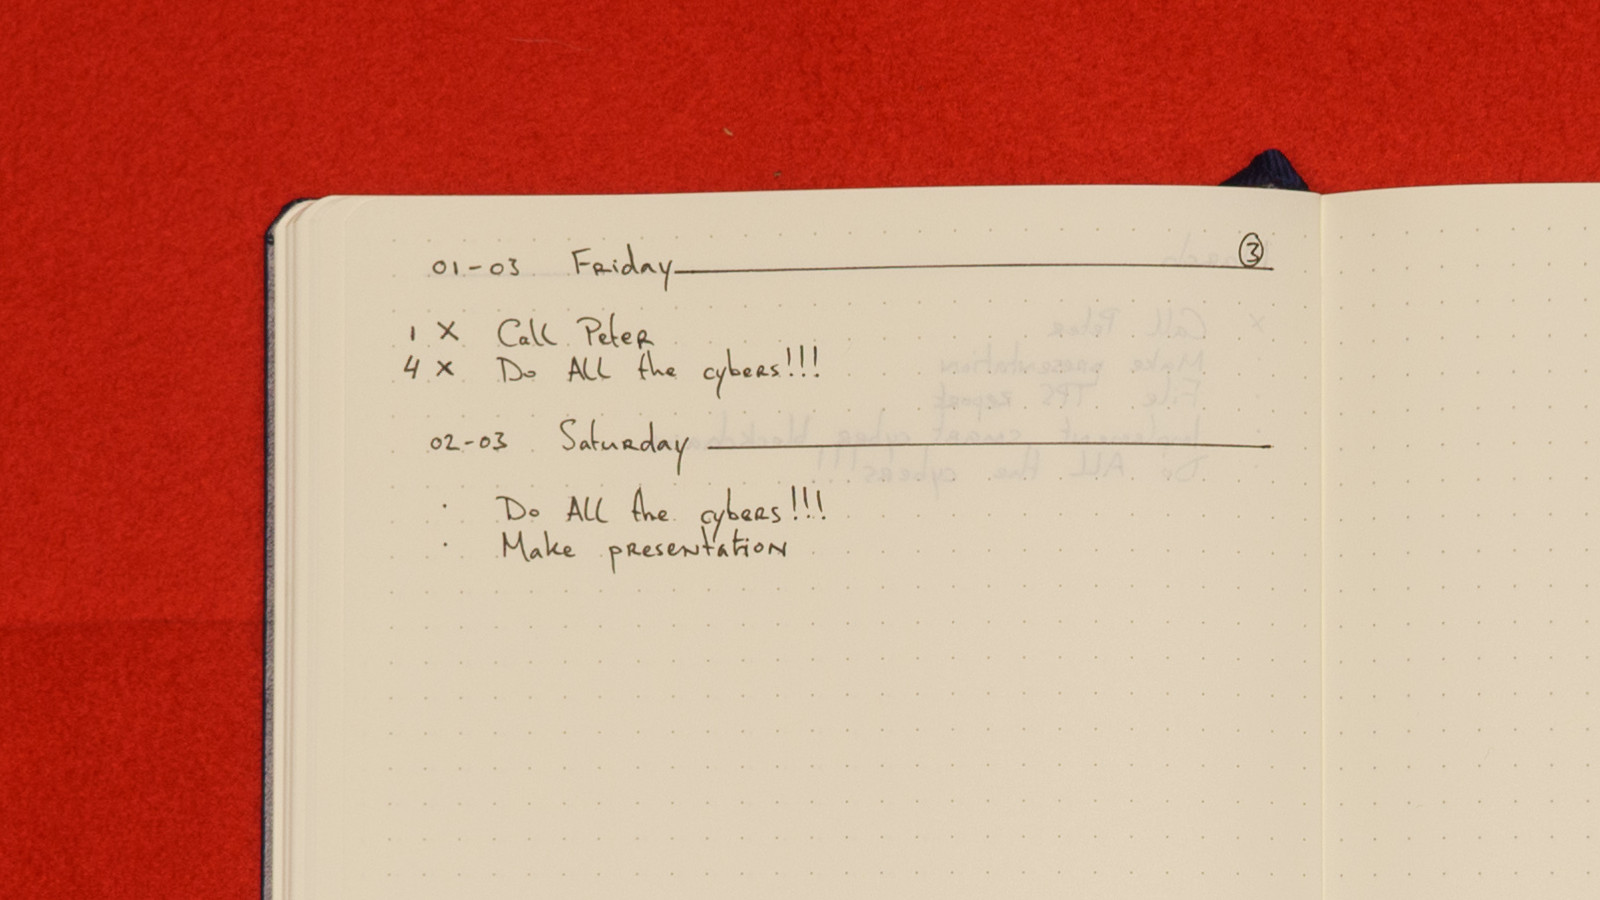
\includegraphics[height=\paperheight]{images/21_daily_log.jpg}}
    \begin{frame}{Daily Log}
    \end{frame}
    }

    {
    \usebackgroundtemplate{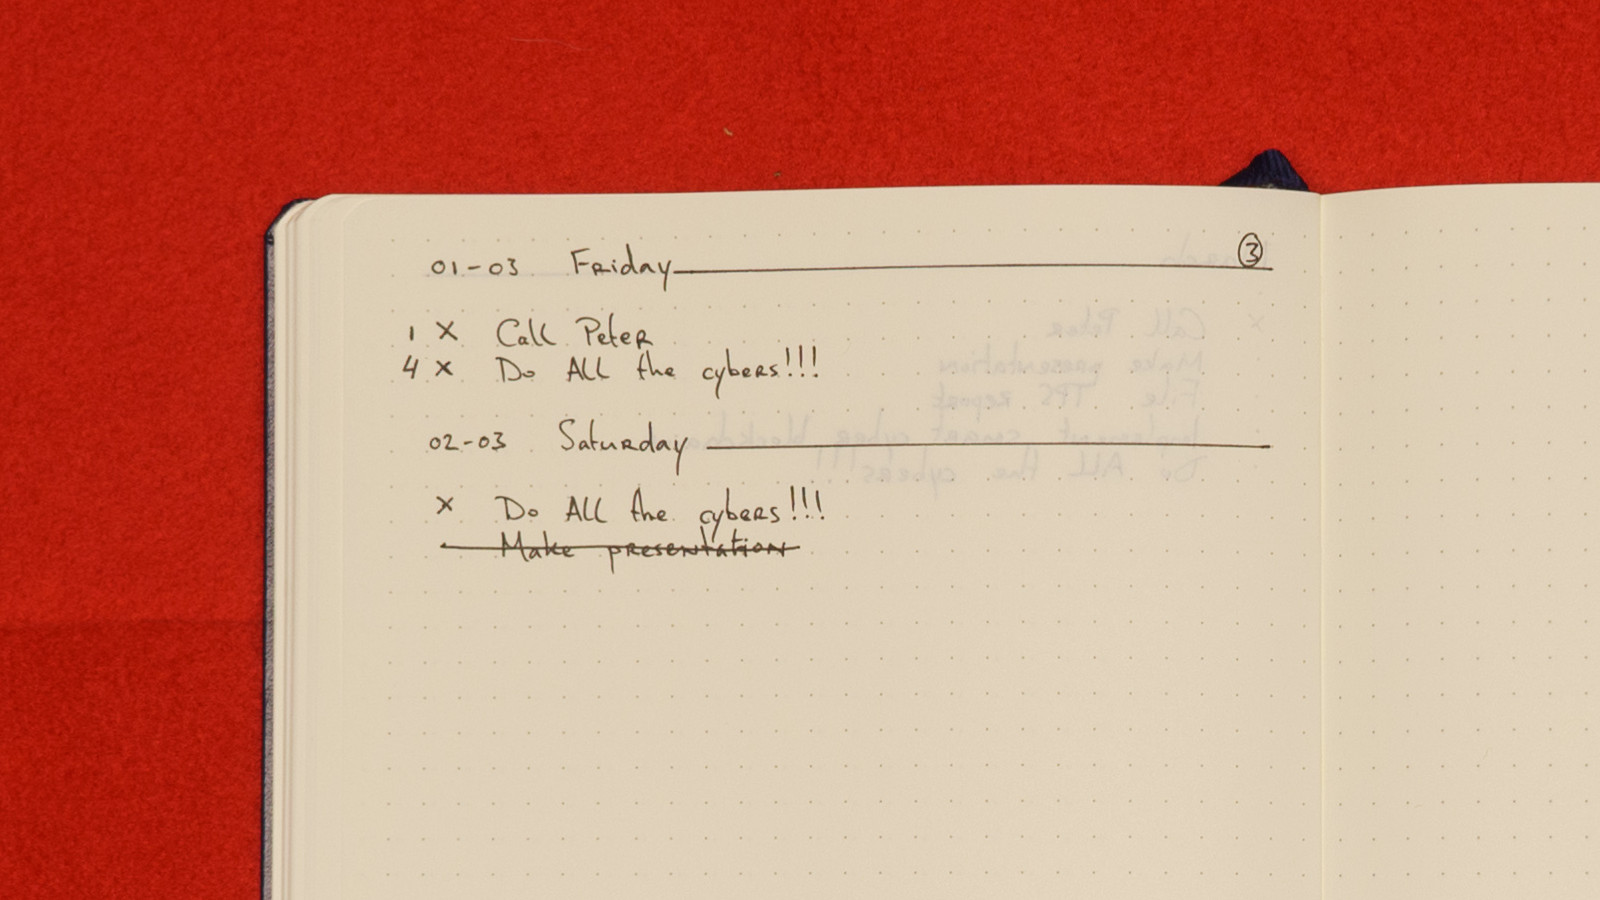
\includegraphics[height=\paperheight]{images/22_daily_log.jpg}}
    \begin{frame}{Daily Log}
    \end{frame}
    }

    {
    \usebackgroundtemplate{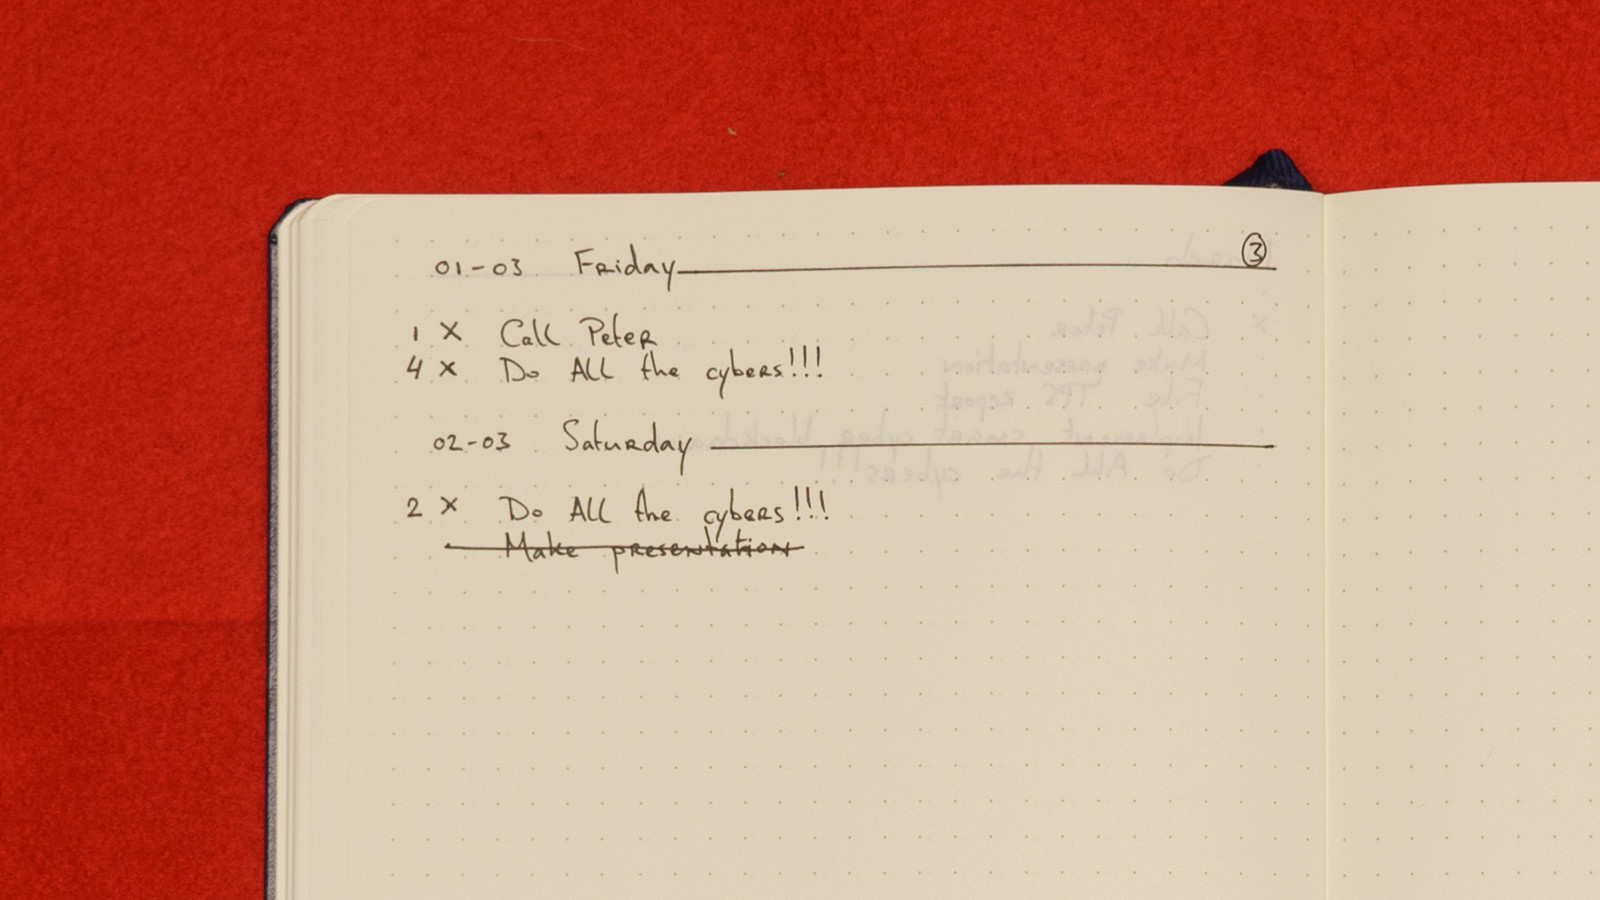
\includegraphics[height=\paperheight]{images/23_daily_log.jpg}}
    \begin{frame}{Daily Log}
    \end{frame}
    }

    {
    \usebackgroundtemplate{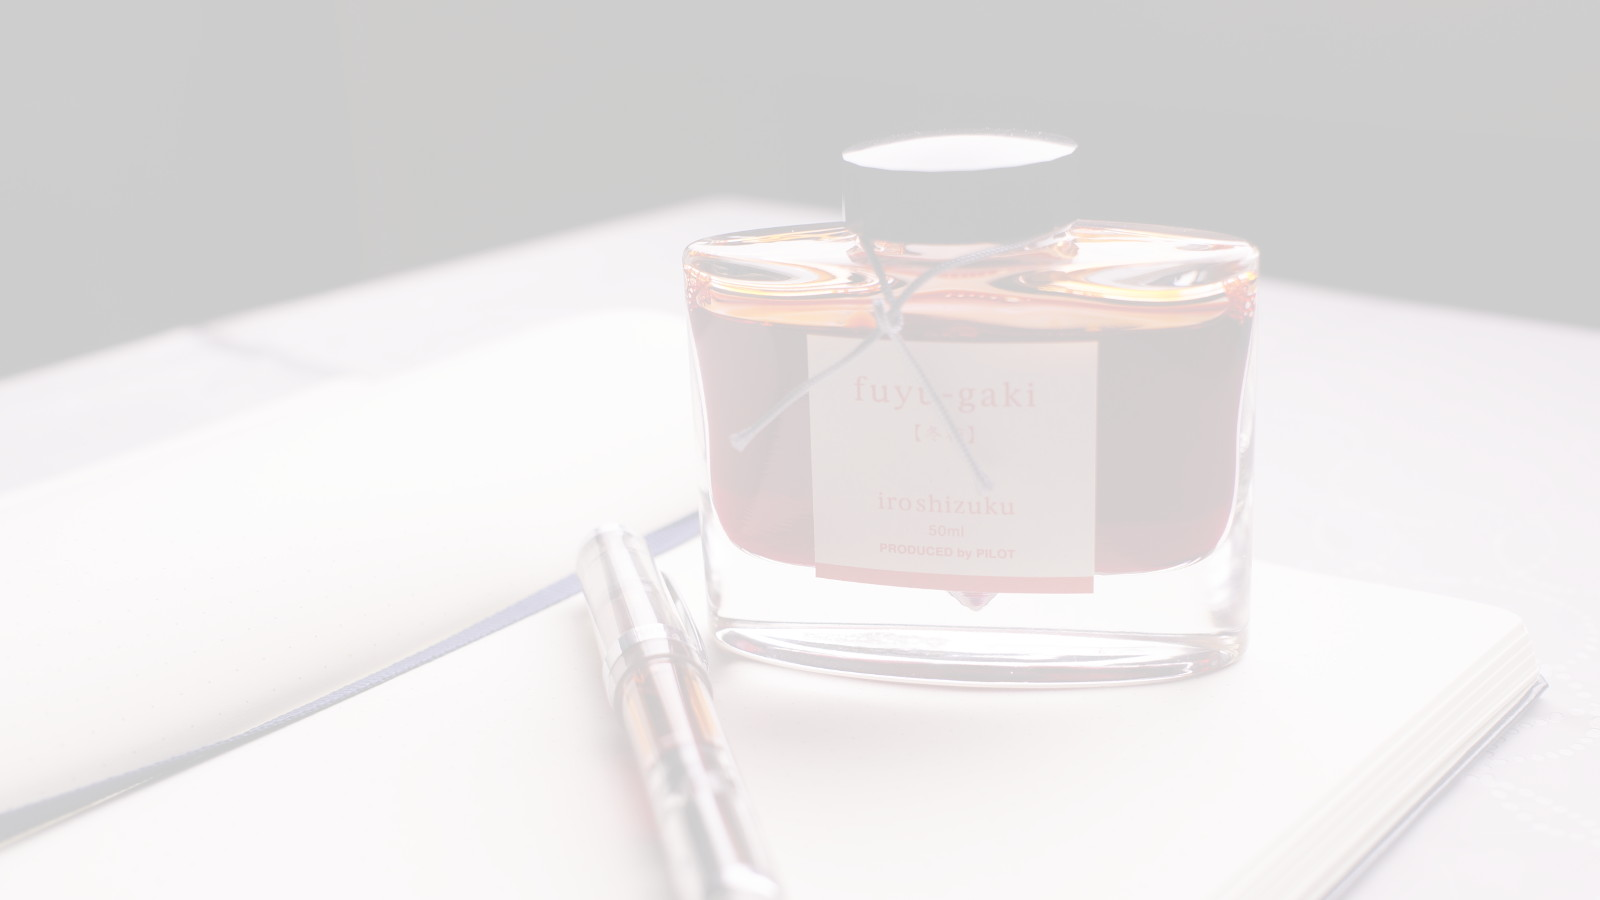
\includegraphics[height=\paperheight]{images/10_notebook_opaque.jpg}}
    \begin{frame}{Migration}
        \begin{itemize}
            \item At the beginning of each month, create a new monthly log
            \item Copy (yes, \alert{copy}!) everything you didn't do last month
            \item Do you still need to do it? If not, get rid of it
            \pause
            \item This helps you focus on what's \alert{really} important
        \end{itemize}
    \end{frame}
    }

    {
    \usebackgroundtemplate{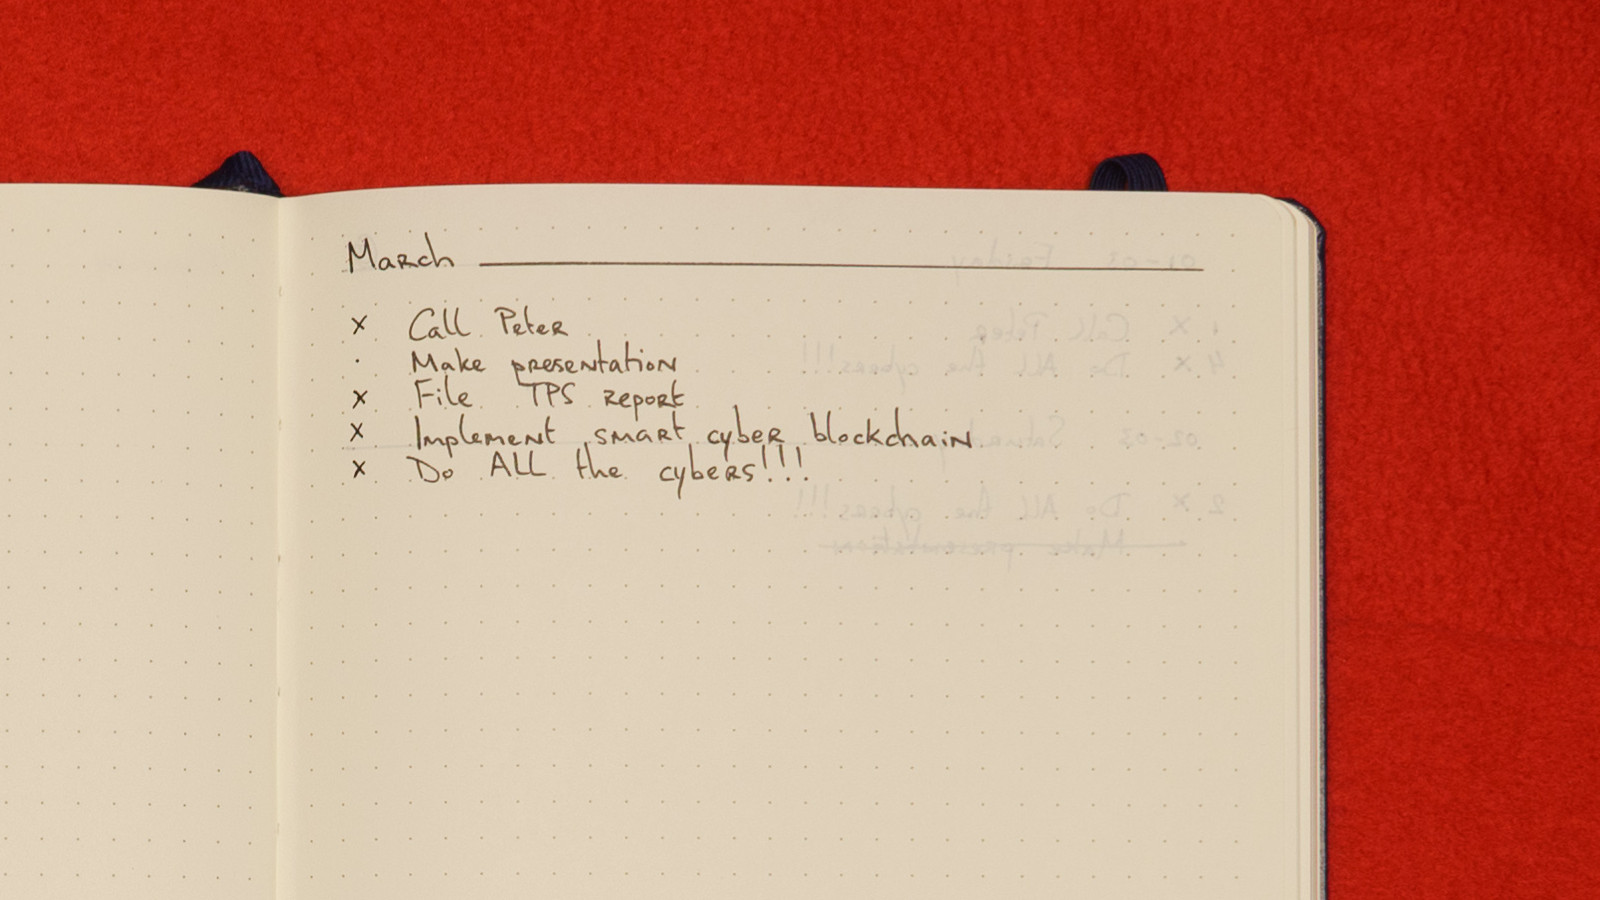
\includegraphics[height=\paperheight]{images/24_monthly_log.jpg}}
    \begin{frame}{Monthly Log}
    \end{frame}
    }

    {
    \usebackgroundtemplate{
\includegraphics[height=\paperheight]{images/25_monthly_log.jpg}}
    \begin{frame}{Monthly Log}
    \end{frame}
    }

    {
    \usebackgroundtemplate{
\includegraphics[height=\paperheight]{images/26_monthly_log.jpg}}
    \begin{frame}{Monthly Log}
    \end{frame}
    }

    {
    \usebackgroundtemplate{
\includegraphics[height=\paperheight]{images/27_monthly_log.jpg}}
    \begin{frame}{Monthly Log}
    \end{frame}
    }

    \section{Conclusion}

    {
    \usebackgroundtemplate{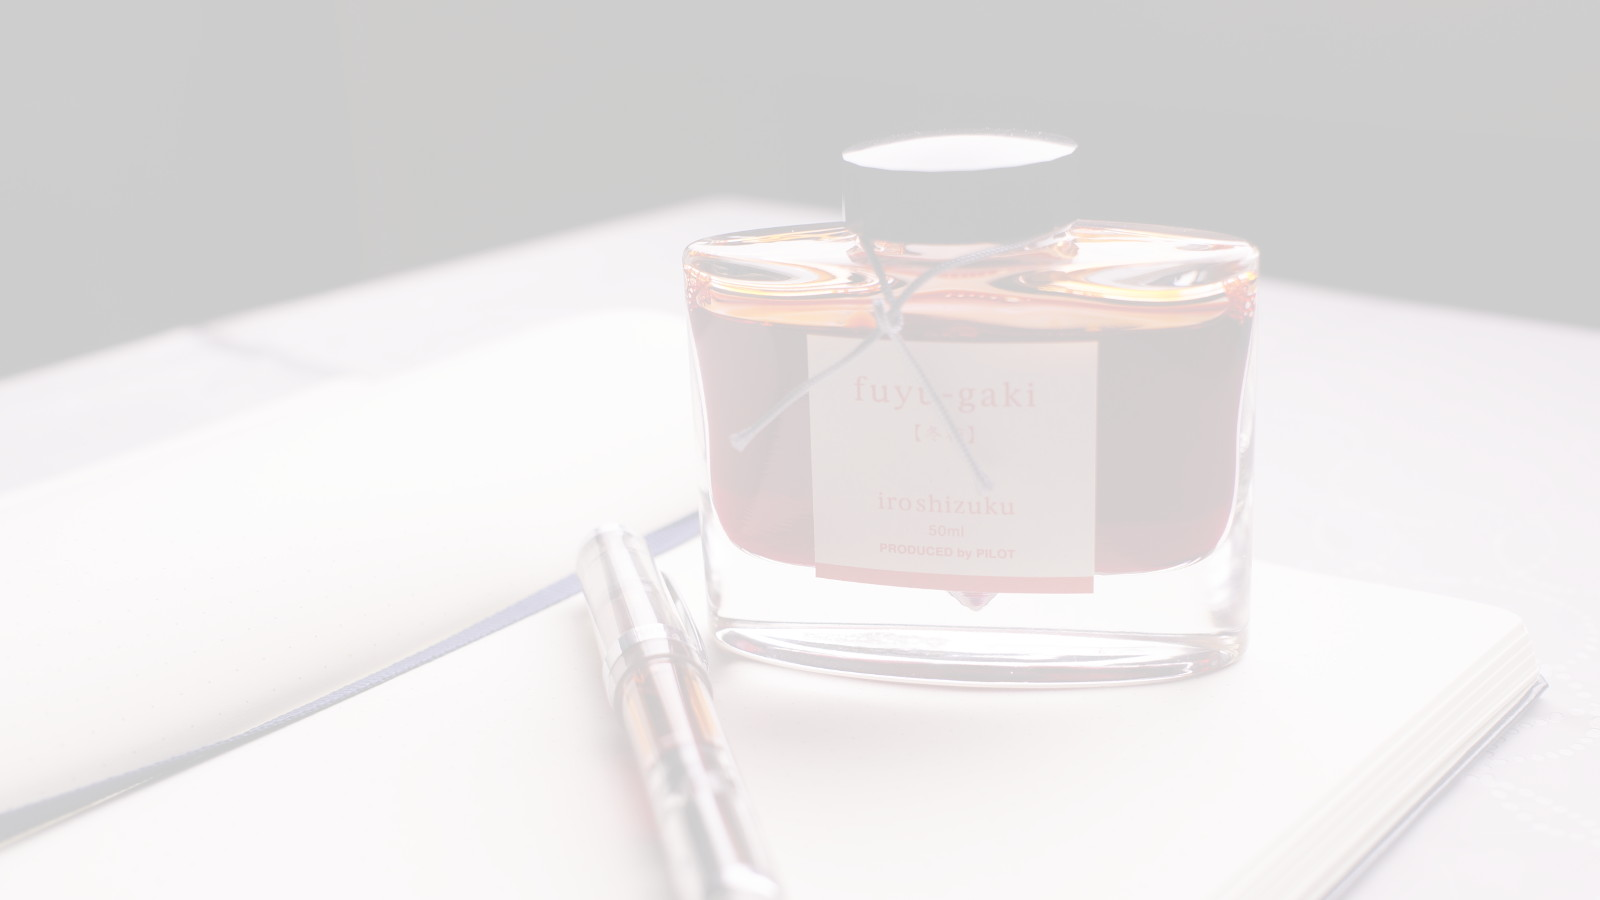
\includegraphics[height=\paperheight]{images/10_notebook_opaque.jpg}}
    \begin{frame}{Conclusion (1)}
        \begin{itemize}
            \item Evaluate what you're doing with your time
            \item Do this monthly (migration), preferably more often
            \item Adjust where required
        \end{itemize}
    \end{frame}
    }

    {
    \usebackgroundtemplate{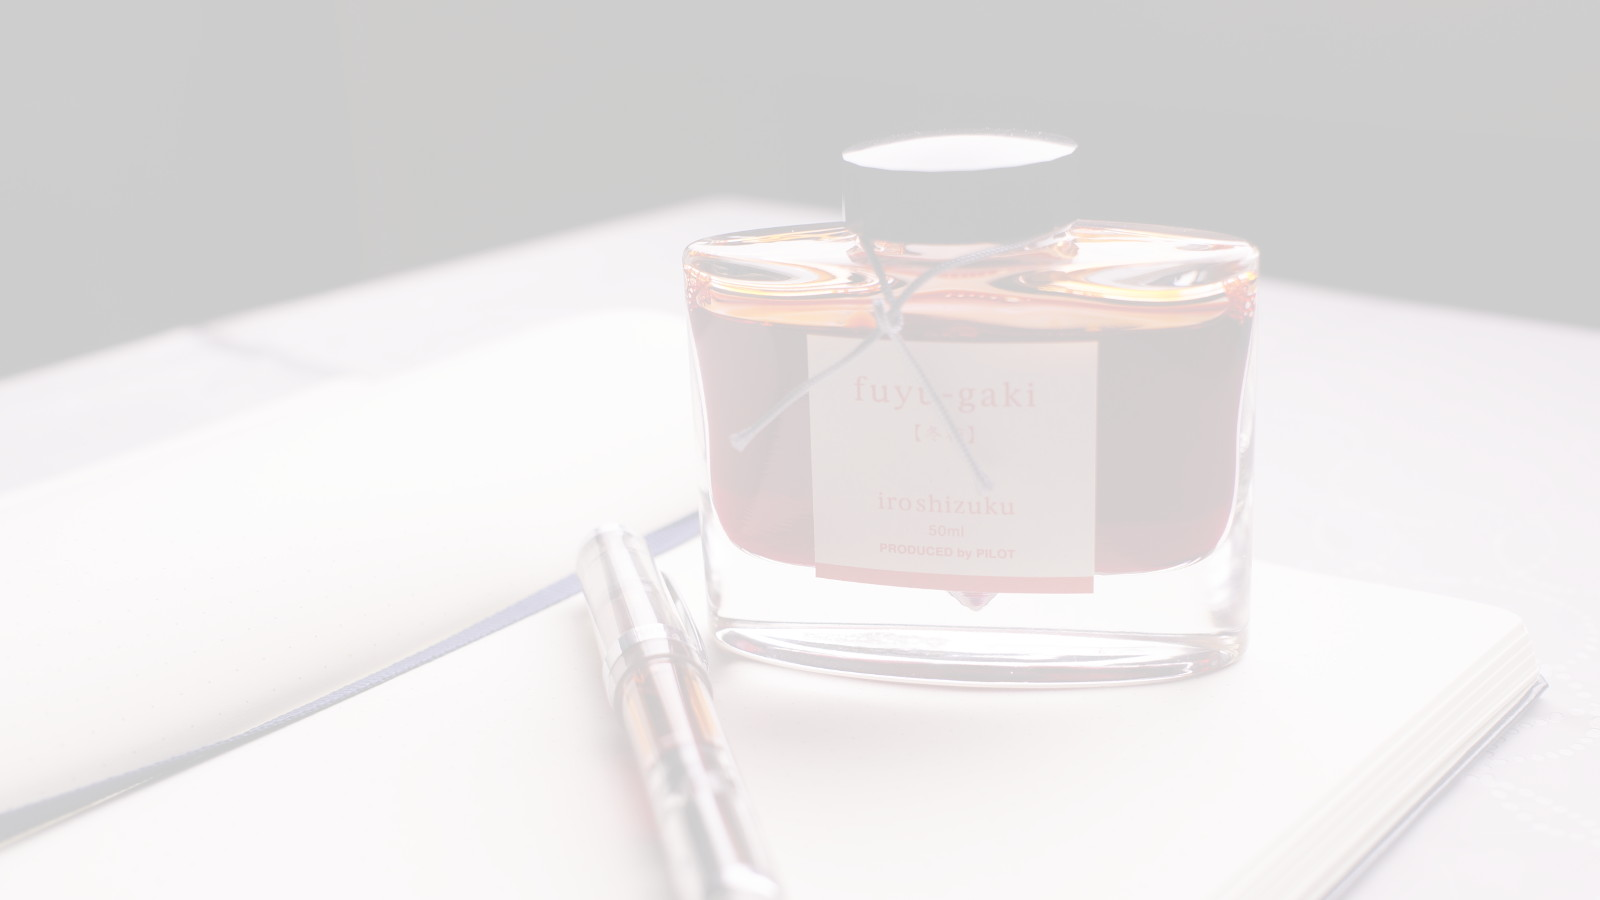
\includegraphics[height=\paperheight]{images/10_notebook_opaque.jpg}}
    \begin{frame}{Conclusion (2)}
        \begin{itemize}
            \item Clears your head, your notebook is your brain now
            \item What if I make a mistake? \pause Cross it out and go again \pause
            \item What if I lose my notebook? \pause Just start over \pause
            \item And there's much more to the Bullet Journal method\ldots{}
        \end{itemize}
    \end{frame}
    }

    {
    \usebackgroundtemplate{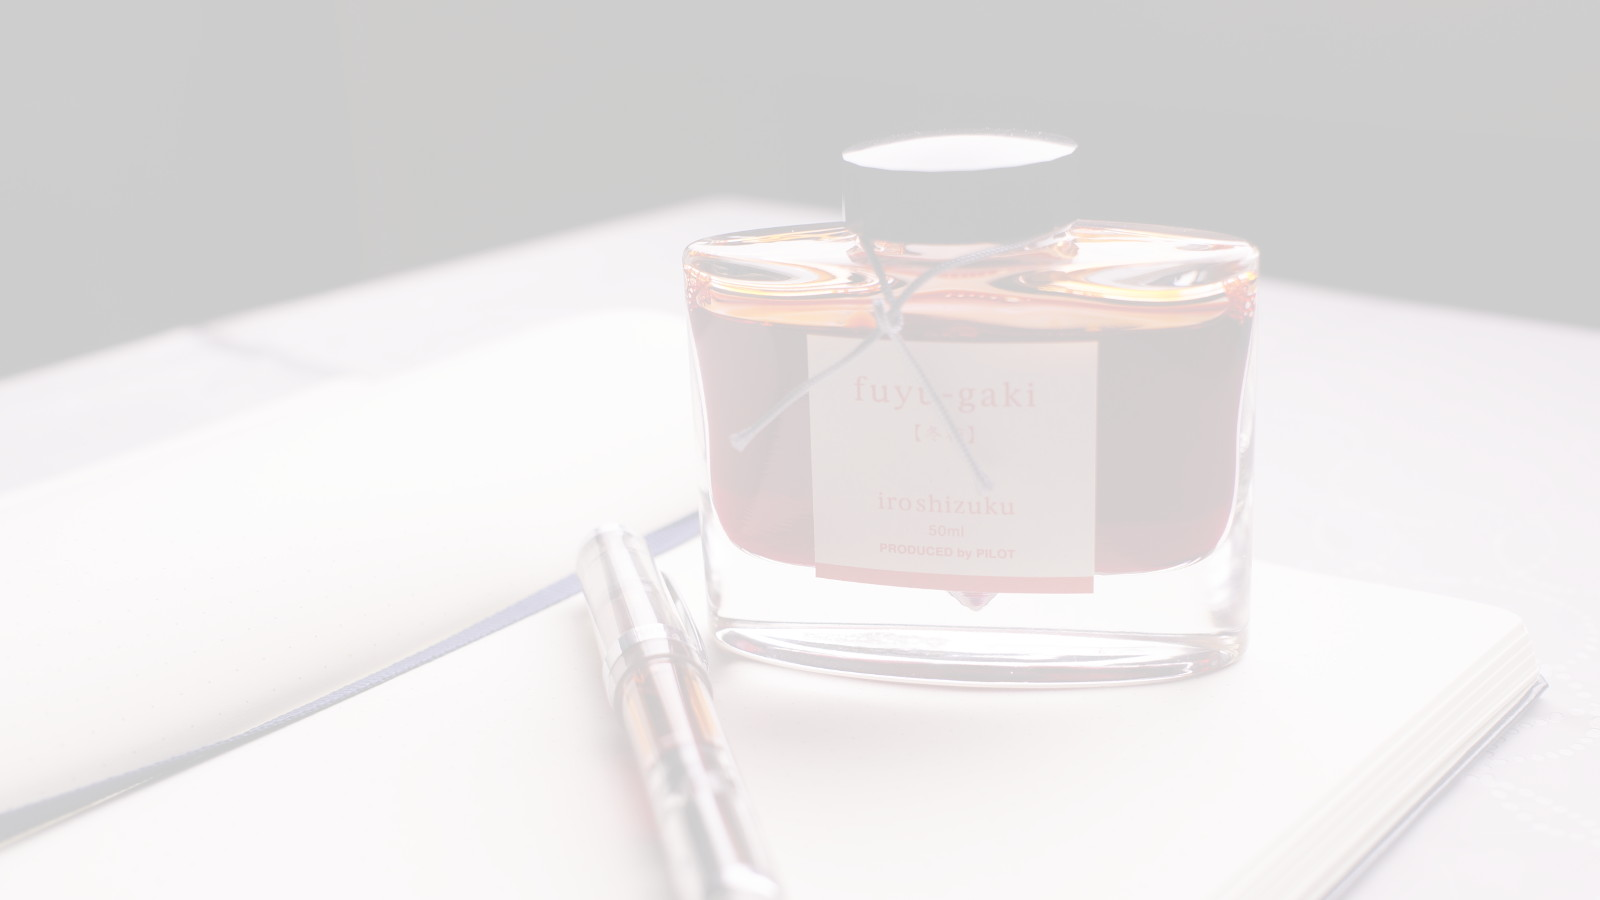
\includegraphics[height=\paperheight]{images/10_notebook_opaque.jpg}}
    \begin{frame}{Caveat Emptor}
        \begin{itemize}
            \item The Bullet Journal method has exploded in popularity recently
            \item Increased focus on `\emph{giving meaning}'
            \item Use the parts that work for you, ignore the rest
        \end{itemize}
    \end{frame}
    }

    \begin{frame}{License}
        Learn more \& Get the source of this presentation from:
        \begin{center}\url{github.com/r1tger/why-so-busy}\end{center}
        Licensed under \href{http://creativecommons.org/licenses/by-sa/4.0/}{Creative Commons Attribution-ShareAlike 4.0}.
        \begin{center}\ccbysa\end{center}
    \end{frame}

    \begin{frame}[standout]
        Questions?
    \end{frame}

    %\appendix

    %\begin{frame}{Collections}
    %\end{frame}

    %{
    %\begin{frame}{Index}
    %\end{frame}
    %}

    %\begin{frame}{Yearly Log}
    %\end{frame}
\end{document}
